\documentclass{beamer}
%Use the [handout] option to eliminate pauses
%\documentclass[handout]{beamer}
%\usetheme{Warsaw}
%\usetheme{Boadilla}
%\usetheme{Madrid}
%\usetheme{Montpellier}
\usetheme{CambridgeUS}

\usepackage{graphicx,amsmath,amssymb,color,multirow, animate}

%\colorlet{newred}{red!60!black}
%\usecolortheme[named=red]{structure}
%\setbeamercolor{block}{bg=white}

%\setbeamertemplate{blocks}{shadow=true}

%\beamertemplatesolidbackgroundcolor{yellow!30}
%\setbeamertemplate{navigation symbols}{}

\begin{document}
%--------------------------------------Title--------------------------------------------------
\title[Extracting and Visualizing Cricket Data]{Extracting and Visualizing Cricket Data Using R}
\author[Niladri \& Mahbub]{Niladri Roy Chowdhury, Mahbubul Majumder}
\institute[Stat. Dept., ISU]{Department of Statistics \\Iowa State University }
\date[\today]{\today}


\begin{frame}
	\maketitle
\end{frame}

\begin{frame}
  \frametitle{Batting and Bowling action}
  
	\begin{columns}
	
		\begin{column}{0.5\textwidth}
			 \begin{center} \scalebox{0.15}{
\includegraphics{bowling.jpg}} \end{center}
		\end{column}
		
		\begin{column}{0.5\textwidth}
			 \begin{center} \scalebox{0.2}{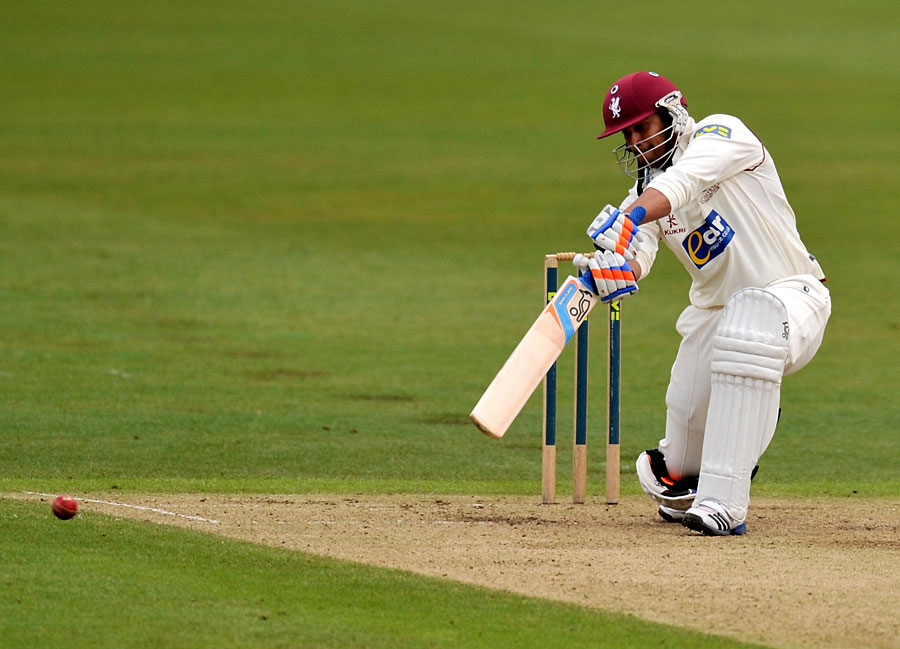
\includegraphics{batting.jpg}} \end{center}
		\end{column}
		
	\end{columns} 
	
\texttt {\tiny picture source: http://www.espncricinfo.com/ci/content/image/561952.html?page=4}	
	
\end{frame}


\begin{frame}
  \frametitle{Statistical graphics}
  
		  \begin{itemize}
			  \item A linear model is fitted to the data.
			  \item $R^2$ = 0.93.
			  \item Is it a good model or a bad model?
			  \item Hold on. Show some plots. We want to see.
			  \item source http://www.espncricinfo.com/ci/content/image/561952.html?page=4
		  \end{itemize}		
\end{frame}

\end{document}

\begin{frame}
  \frametitle{We want to see}
  
	\begin{columns}
	
		\begin{column}{0.5\textwidth}
		  \begin{itemize}
			  \item This residual plot shows the problem with the model.
			  \item Statistical graphics have been used for
			     \begin{itemize}
			        \item exploratory data analysis.
			        \item model checking and diagnostics.
           \end{itemize}				  
			  \item Can we use statistical graphics for inference?
		  \end{itemize}		
		\end{column}
		
		\begin{column}{0.5\textwidth}
			 \begin{center} \scalebox{0.35}{\includegraphics{residual_plot.pdf}} \end{center}
		\end{column}
		
	\end{columns} 
	
\end{frame}


\begin{frame}
\frametitle{Statistical graphics}
  \begin{itemize}
    \item Buja et al (2009)
		  \begin{itemize}
			  \item Introduced method to test the significance of findings.
			  \item Their focus was on testing overall model fitting.
		  \end{itemize}
		\item Some times we are particularly interested in model parameters.
		\item This presentation focuses on testing parameters related to regression models. 
  \end{itemize}		  
\end{frame}


\begin{frame}
  \frametitle{Test Statistic}
  
	\begin{columns}
	
		\begin{column}{0.5\textwidth}
		  \begin{itemize}
			  \item Function $T(Y)$ that maps data $Y$ to a plot.
			  \item Associated with a specific null hypothesis.
			  \item A good test statistic should display an extreme feature of the data if it exists.
			  \item As an example, this test statistic investigates the existence of a non-zero slope.
			  \item Testing $H_0:$ Slope=0 vs $H_1:$ Slope $\ne 0$
		  \end{itemize}		
		\end{column}
		
		\begin{column}{0.5\textwidth}
			 \begin{center} \scalebox{0.35}{\includegraphics{stat_intercept.pdf}} \end{center}
		\end{column}
		
	\end{columns} 
	
\end{frame}



\begin{frame}
  \frametitle{Compare test statistic with null distribution}
	\begin{columns}
		\begin{column}{0.4\textwidth} Lineup plot
		  \begin{itemize}
			  \item A layout of $a$x$b$ plots.
			  \item One of the plots is of observed data
			  \item All other plots are simulated from null model.
			  \item Reject null hypothesis if observed plot is identified.
			  \item To identify the observed plot, more than one person can be involved.
		  \end{itemize}		
			
		\end{column}
		
		\begin{column}{0.6\textwidth}
			 \begin{center} \scalebox{0.45}{\includegraphics{test_slope.pdf}} \end{center}
		\end{column}
	\end{columns}  
\end{frame}



\begin{frame}
  \frametitle{Comparison: Visual vs Mathematical Inference}
  Model: $Y = \beta_0 + \beta X + \epsilon $; $\epsilon \stackrel{iid}{\sim} N(0,\sigma^2)$ 
  {\small
  \begin{table}[ht] 
		\begin{tabular}{llll} 
			\hline
				   & Mathematical Inference &  Visual Inference \\ %[0.5ex] % inserts table %heading 
			\hline
				  Hypothesis & $H_0: \beta=0$ vs $H_1: \beta \ne 0$& $H_0: \beta=0$ vs $H_1: \beta \ne 0$\\

				 & \begin{minipage}[h]{1cm} \begin{center} \scalebox{0.18}{\includegraphics{down_arrow.pdf}} \end{center} \end{minipage} & \begin{minipage}[h]{1cm} \begin{center} \scalebox{0.18}{\includegraphics{down_arrow.pdf}} \end{center} \end{minipage} \\
				  
				 Test statistic & $T(y)=\frac{\hat{\beta}}{se(\hat{\beta})}$ & $T(y)=$ \begin{minipage}[h]{1cm} \begin{center} \scalebox{0.08}{\includegraphics{stat_intercept.pdf}} \end{center} \end{minipage} \\
				 
				 & \begin{minipage}[h]{1cm} \begin{center} \scalebox{0.18}{\includegraphics{down_arrow.pdf}} \end{center} \end{minipage} & \begin{minipage}[h]{1cm} \begin{center} \scalebox{0.18}{\includegraphics{down_arrow.pdf}} \end{center} \end{minipage} \\
				 
				 Null Distribution & $f_{T(y)}(t); $\begin{minipage}[h]{1cm} \begin{center} \scalebox{0.08}{\includegraphics{stat_mathematical_test.pdf}} \end{center} \end{minipage} & $f_{T(y)}(t); $ \begin{minipage}[h]{1cm} \begin{center} \scalebox{0.08}{\includegraphics{test_slope.pdf}} \end{center} \end{minipage} \\

				 & \begin{minipage}[h]{1cm} \begin{center} \scalebox{0.18}{\includegraphics{down_arrow.pdf}} \end{center} \end{minipage} & \begin{minipage}[h]{1cm} \begin{center} \scalebox{0.18}{\includegraphics{down_arrow.pdf}} \end{center} \end{minipage} \\
				 
				 
				 Reject $H_0$ if & observed $T$ is extreme & observed plot is identifiable \\
			\hline 
		\end{tabular}
	\end{table}	
	}
\end{frame} 




\begin{frame}
  \frametitle{P value and Type-I error}
	For a lineup of $m$ plots
	\begin{enumerate}
	\item p-value for an Individual evaluation
		\begin{itemize}
			\item When reject report p-value $\le \frac1m$ .
			\item When cannot reject report p-value $\ge 1-\frac1m$ .
		\end{itemize}
	\item p-value for $N$ independent evaluations
		\begin{itemize}
		  \item Under Null hypothesis, $Pr$(Reject)=$\frac1m$ for each evaluation.
			\item number of success $ U \sim Binom(N,\frac1m)$.
			\item p-value= $Pr(U \ge u)= \sum_{k \ge u}^N {{N \choose k} (\frac1m)^k(1-\frac1m)^{(N-k)}}$ where $u$ be the observed number of success.
			\item Exact probability for discrete variable makes it conservative.
			\item When $N=1$ this p-value matches with individual judgment p-value
		\end{itemize}
	\item Type-I error probability = $\frac1m$.
	\end{enumerate}
\end{frame}




\begin{frame}
\frametitle{$Y_i = \beta_0 + \beta_1 X_{i1} + \beta_2 X_{i2}+ \beta_3 X_{i1} X_{i2}+ ... + \epsilon_i $ ; $\epsilon_i \stackrel{iid}{\sim} N(0,\sigma^2)$}

{\footnotesize
\begin{table}[ht] 
	\centering 
		%\begin{tabular}{m{3cm}m{2.5cm}m{2.6cm}m{5.5cm}} 
		\begin{tabular}{lll} 
			\hline
				Null Hypothesis & Type &  Test Statistic   \\ %[0.5ex] % inserts table %heading 
			\hline 
								$H_0: \beta_k=0$ & Residual Plot & \begin{minipage}[h]{1cm}\begin{center}  	\scalebox{0.081}{\includegraphics{stat_bet_p.pdf}} \end{center} \end{minipage}  \\ 
				
				$H_0: X$ Linear & Residual Plot & \begin{minipage}[h]{1cm}\begin{center}   \scalebox{0.081}{\includegraphics{stat_nonlinear.pdf}} \end{center} \end{minipage} \\ 

				\begin{minipage}[h]{4cm} $H_0: \beta_k=0$ for categorical $X_k$ \end{minipage} & Boxplot & \begin{minipage}[h]{1cm}\begin{center}  \scalebox{0.081}{\includegraphics{stat_category.pdf}} \end{center} \end{minipage}  \\ 
								
				\begin{minipage}[h]{4cm} $H_0: \beta_k=0$ (interaction 
with categorical $X_k$) \end{minipage} & Scatter plot & \begin{minipage}[h]{1cm}\begin{center} \scalebox{0.081}{\includegraphics{stat_interection.pdf}} \end{center} \end{minipage}\\				

				$H_0:$ Model Fits & Histogram & \begin{minipage}[h]{1cm}\begin{center}  \scalebox{0.081}{\includegraphics{stat_goodness_simple.pdf}} \end{center} \end{minipage} \\[.5ex] % [1ex] adds vertical space 
			\hline 
		\end{tabular} 
	\label{tbl:stat_simple} 
\end{table} 		
}
\end{frame}



\begin{frame}
  \frametitle{Power for testing $H_0: \theta \in \Theta_0$ vs $H_1: \theta \in \Theta^c_0$}
  \begin{itemize}
    \item For a lineup of $m$ plots, power function of $\theta$ be defined as 
    \begin{equation*}
      \beta(\theta)= 
        \begin{cases} 
              \text{Type-I error}=\frac1m & \text{if $\theta \in \Theta_0$,} \\
              Pr(\text{Reject } H_0) &\text{if $\theta \in \Theta^c_0$.}
        \end{cases}
    \end{equation*}
    \item Estimated power = $\frac uN$ \\
             $u$ = number of successful evaluations \\
             $N$ = number of independent evaluations. 
    \item A generalized mixed linear model can be used to estimate power. 
  \end{itemize}

\end{frame}


\begin{frame}
  \frametitle{Simulation based experiment}
  \begin{itemize}
    \item Model: $Y = \beta_0 + \beta_1 X_1 + \beta_2 X_2 + \epsilon $; $\epsilon \stackrel{iid}{\sim} N(0,\sigma^2)$; $X_2$ categorical
    \item Hypothesis $H_0: \beta_2=0$ vs $H_1: \beta_2 \ne 0$
    \item Test statistic is the boxplot of residuals of fitted null model grouped by $X_2$. For lineup plot we simulate data from $N(0,\hat{\sigma}^2)$
  \end{itemize}
  \begin{center} \scalebox{0.25}{\includegraphics{stat_category.pdf}} \end{center}
\end{frame}


%\begin{frame}
%  \frametitle{Procedure for the experiment}
%    Flow of the experiment
%      \begin{itemize}
%        \item Simulate data from the linear model for specific parameters and call it observed data.
%        \item fit null model to the observed data and obtain parameter estimates.
%        \item Obtain null distribution for that specific parameter settings.
%        \item Present the null distribution plot to individual people to see if they can identify the observed plot.
%      \end{itemize}
%\end{frame}


\begin{frame}
  \frametitle{Survey Setting}      
      \begin{itemize}    
        \item Values of parameters considered for survey experiment.
\begin{table}[hbtp]
%\caption{Values of parameters considered for survey experiment} % title name of the table
\centering
\begin{tabular}{c c r r r r r }
\hline
Sample size ($n$) & $\sigma$ &\multicolumn{5}{c}{values for $\beta_2$}
\\ [0.5ex]
\hline
&  5 & 0 & 1 & 3 & 5 & 8  \\[-1ex]
\raisebox{1.5ex}{100} &12
& 1 & 3 & 8 & 10 & 16  \\[1ex]
&  5 & 0 & 1 & 2 & 3 & 5  \\[-1ex]
\raisebox{1.5ex}{300} & 12
& 1 & 3 & 5 & 7 & 10  \\[1ex]
\hline
\end{tabular}
\label{tbl:expeiment_params}
\end{table} 
        \item For each of the above combinations 3 independent lineup plots were generated.
        \item Recruited 324 participants through Amazon Mechanical Turk web site. 
      \end{itemize}    
\end{frame}

%\begin{frame}[containsverbatim]
%  \frametitle{Demonstration of data collection from web}
%  \begin{verbatim}
%    http://www.public.iastate.edu/~mahbub/feedback
%  \end{verbatim}
%\end{frame}



\begin{frame}
  \frametitle{Survey results}
	\begin{columns}
		\begin{column}{0.45\textwidth}
		  \begin{itemize}
			  \item Sample size 100, $\beta=1$ and $\sigma=5$.
			  \item For observed plot, p-value is 0.75
			  \item Most of the responses are 18. Has p-value 0.028 which is minimum. 
			  \item Attempted 18 times with 5.5\% success.
		  \end{itemize}		
			
		\end{column}
		
		\begin{column}{0.55\textwidth}
			 \begin{center} \scalebox{0.4}{\includegraphics{plot_100_1_5_3.pdf}} \end{center}
		\end{column}
	\end{columns}  
\end{frame} 


\begin{frame}
  \frametitle{Survey results}
	\begin{columns}
		\begin{column}{0.45\textwidth}
		  \begin{itemize}
			  \item Sample size 300, $\beta=5$ and $\sigma=5$.
			  \item For observed plot, p-value $ < 0.0001$
			  \item Attempted 23 times with 100\% success.
		  \end{itemize}		
			
		\end{column}
		
		\begin{column}{0.55\textwidth}
			 \begin{center} \scalebox{0.4}{\includegraphics{plot_300_5_5_1.pdf}} \end{center}
		\end{column}
	\end{columns}  
\end{frame} 

\begin{frame}
  \frametitle{Expected power}
        \begin{itemize}
             \item Under $H_1$ distribution of p-value $p_m$ is right skewed
             \item Under $H_0$ $p_m \sim $ Uniform(0,1)
             \item $p_0 = min(p_m) \sim beta(1,m-1)$
             \item Expected power = $Pr(p_{obs} < p_0)$
        \end{itemize}	
			 \begin{center} \scalebox{0.45}{\includegraphics{power_expected.pdf}} \end{center}
\end{frame} 

\begin{frame}
  \frametitle{Observed power}
  \begin{center}  	\scalebox{0.5}{\includegraphics{power_observed.pdf}} \end{center}
\end{frame}

\begin{frame}
  \frametitle{Power estimated from logistic model}
  Sample size = 100, standard deviation = 12
  \begin{center}  	\scalebox{0.5}{\includegraphics{power_model.pdf}} \end{center}
\end{frame}

\begin{frame}
  \frametitle{Power estimated from generalized mixed model}
  Sample size = 100, standard deviation = 12
  \begin{center}  	\scalebox{0.55}{\includegraphics{power_subject.pdf}} \end{center}
\end{frame}


\begin{frame}
  \frametitle{Future work}
  \begin{itemize}
    \item Visual inference is not the competitor to traditional inference.
    \item May use where traditional tests can't be used.
  \end{itemize}
      
  \begin{itemize}
    \item What if not normal?
      \begin{itemize}
        \item Extend this study for generalized linear model.
      \end{itemize}
    \item Apply the procedure with real data. 
    \item Conduct survey   
      \begin{itemize}
        \item Examine the other test statistics.
        \item Asses the sensitivity of power to modeling conditions.
        \item Discover the most effective specification of a plot.
      \end{itemize}    
  \end{itemize}
\end{frame}

\begin{frame}
  \frametitle{Thanks}
  \begin{center} Question? \end{center}
\end{frame}

\end{document}



%==============================================================================================


